\documentclass[12pt]{article}
\usepackage[utf8]{inputenc}
\usepackage{graphicx}
\usepackage{float}
\usepackage{amsmath}
\usepackage{amsthm}
\usepackage{bm}
\usepackage[nottoc]{tocbibind}
\usepackage{accents}
\usepackage{bookmark}
\newcommand{\ubar}[1]{\underaccent{\bar}{#1}}


\usepackage[natbibapa]{apacite}
%\renewcommand{\BBAA}{and}

\title{An Introduction to Other-Regarding Preferences With an Application to Contract Design}
\author{João Eira}
\date{Janeiro 2018}


\setcounter{secnumdepth}{5}


\newtheorem{theorem}{Theorem}[section]
\newtheorem{corollary}{Corollary}[theorem]
\newtheorem{lemma}[theorem]{Lemma}
\newtheorem{prop}{Proposition}
\newtheorem{definition}{Definition}


\let\oldquote\quote
\let\endoldquote\endquote
\renewenvironment{quote}[2][]
{\if\relax\detokenize{#1}\relax
	\def\quoteauthor{#2}%
	\else
	\def\quoteauthor{#2~---~#1}%
	\fi
	\oldquote}
{\par\nobreak\smallskip\hfill\quoteauthor%
	\endoldquote\addvspace{\bigskipamount}}


\newenvironment{dedication}
  {\clearpage           % we want a new page
   \thispagestyle{empty}% no header and footer
   \vspace*{\stretch{1}}% some space at the top 
   \itshape             % the text is in italics
   \centering         % flush to the right margin
  }
  {\par % end the paragraph
   \vspace{\stretch{3}} % space at bottom is three times that at the top
   \clearpage           % finish off the page
}


\newenvironment{agradecimentos}
  {\clearpage           % we want a new page
   \thispagestyle{empty}% no header and footer
   \vspace*{\stretch{1}}% some space at the top 
   \raggedright         % flush to the left margin
  }
  {\par % end the paragraph
   \vspace{\stretch{3}} % space at bottom is three times that at the top
   \clearpage           % finish off the page
}


\begin{document}
\pagenumbering{roman} %this part doesn't really count for the counting 
\begin{dedication}
Para a Rita, que me atura, e para os meus pais, que me criaram, algo que a Rita pode ou não achar ter sido uma má decisão.
\end{dedication}
\newpage
%\begin{agradecimentos}
%[agradecimentos]
%\end{agradecimentos}
\newpage
\section*{Resumo}
Os modelos económicos de comportamento individual supõem, frequentemente, que na avaliação entre alternativas concorrentes os agentes apenas estão preocupados com a forma como cada alternativa os afeta pessoalmente. Esta simples e razoável suposição postula que os agentes cuidam apenas do interesse próprio (egoísmo racional), não se preocupando com o possível impacto das suas decisões sobre aqueles com quem interagem. O presente trabalho desafia esta suposição.

Ao longo das últimas décadas foi possível observar a acumulação de resultados experimentais provenientes de jogos como o ultimato e o \textit{gift exchange}, onde o comportamento não é explicável com base em preferências puramente egoístas. Com efeito, os agentes geralmente tomam decisões que reduzem o seu bem-estar, desde que ao fazê-lo os restantes agentes possam beneficiar. Neste caso, em contraste com o puro interesse próprio, os agentes são ditos possuírem preferências sociais. Estes agentes estarão pois não são só preocupados com o que lhes acontece mas também com o que acontece aos outros agentes.

Uma larga parte dos resultados experimentais discutidos neste trabalho foram obtidos através do uso de experiências laboratoriais. A questão da validade externa destes resultados tem sido um ponto de disputa. As experiências laboratoriais são realizadas em ambientes altamente artificiais onde são colocadas fortes restrições no comportamento dos participantes. Embora isto lhes imbua com a sua fonte de força metodológica, é também uma fraqueza. Os resultados provenientes de experiências laboratoriais não generalizam necessariamente para o mundo real, e estes são frequentemente comparados com os resultados obtidos através de trabalho de campo devido à suposta maior validade externa destes últimos. A questão da validade externa das experiências laboratoriais é examinada e conclui-se que estas são uma ferramenta valida para a acumulação de evidência cientifica sobre o comportamento humano.

A aversão à desigualdade, é apresentada como um método de modelar preferências sociais. O modelo proposto é utilizado então para explicar o comportamento observado (em laboratório) no jogo do ultimato. Um exemplo sobre como utilizar preferências sociais, para estudar interações económicas no mundo real, é analisado na sua aplicação ao estudo da formulação de contratos sob risco moral.
\\

\noindent
\textbf{Classificação JEL:} D01; C70; B41.

\newpage
\section*{Abstract}
Economic models of individual behavior often make the assumption that in evaluating between competing alternatives agents are only concerned with how each alternative impacts their own payoffs. This simple, yet reasonable, assumption postulates that agents are self-regarding, that is, agents are not concerned with how their decisions affects other people. This study casts doubt over this assumption. 

Over the last several decades there has been a steady accumulation of experimental evidence from games such as the ultimatum game and the gift exchange game where the observed behavior is not explained by assuming that agents have self-regarding preferences. Agents often make decisions that lower their payoff if by doing so other agents are better off. In contrast to self-regarding preferences, agents are said in this case to have other-regarding preferences. They are not only preoccupied with themselves but also with other people. 

Most of the evidence discussed in this study was gathered through the use of laboratory experiments. The issue of the external validity of this evidence has long been a point of contention. Laboratory experiments are highly artificial environments that place strong constraints on individual behavior. While this imbues them with their source of methodological strength, it is also a weakness. Evidence gathered in the laboratory need not generalize to the real world, and laboratory experiments are often compared with field studies which purport to provide evidence that is more externally valid. We examine the question of the external validity of laboratory experiments and conclude they are a valid tool for the gathering of scientific evidence about human behavior. 

Inequity aversion is presented as a method of modeling other-regarding preferences. The model is promptly used to explain the behavior documented in the ultimatum game. An example on how to use other-regarding preferences to study real world economic interactions is provided in the study of contract design under moral hazard.
\\

\noindent
\textbf{JEL Classification:} D01; C70; B41.
% D01 	Microeconomic Behavior: Underlying Principles 
% C70 	Game Theory and Bargaining Theory - General 
% B41 	Economic Methodology 
% C90   Design of Experiments - General
% D86 	Economics of Contract: Theory 
	
\newpage

\renewcommand{\contentsname}{Table of Contents}
\begin{center}
\tableofcontents
\end{center}


\newpage

\setcounter{page}{1} %so that it starts in 1
\pagenumbering{arabic} %arabic numerals
\section{Introduction}
Economics is a \textit{social} science and the economic behavior that is its subject of study is \textit{human} behavior. As social scientists, economists are interested in studying agents, their actions, the reasons behind them, and the consequences that result from them. It is through the use of tractable models that economists perform their studies and, as a necessary step to develop these models, it is required that the goals and motivations that precede and drive human behavior be formalized. 

We are regularly faced with situations where we have to choose between multiple possible courses of action. Before entering college we must decide between majoring in Physics or Economics. When lunch hour arrives, and we find ourselves at a mall, we have to choose one restaurant out from possible dozens. Economists deal with this basic fact of everyday life by introducing the concept of preferences, which are defined as rankings that express the subjective comparative evaluations of alternatives \citep{hausman2011preference}. 

An agent's behavior can be summarized as the maximization of an abstract utility function. While this utility function does not necessarily take into account the underlying psychological processes that underlie preference formation, it has become standard in Economics to take this function as being the result of an evaluation that takes into account as its sole parameter how each alternative impacts the agent's payoff. Under this behavioral assumption, the maximizing behavior corresponds to the idea that in the presence of competing alternatives people seek to maximize their own expected payoffs. Agents are then said to be self-regarding.

This assumption was put forth in 1881, when the political economist and philosopher Francis Edgeworth asserted that "the first principle of Economics is that every agent is actuated only by self-interest" \citep{edgeworth1881mathematical}. More famously, we see it in Adam Smith's concept of the invisible hand, where the market is able to turn what are private vices into public virtues.\footnote{Contrary to what one might infer from the Invisible Hand concept, Adam Smith never believed humans are only driven by self-interest \citep{smith1822theory}.} 

This work intends to show that there is sufficient experimental evidence showing that the assumption that agents are self-regarding is insufficient. It will be shown that there is a wide range of behavior which the self-regarding assumption is not able to explain and that instead one needs to take into account that agents are concerned not only with themselves but also take into account the well-being of others.

We will therefore contrast \textit{other-regarding preferences} with \textit{self-regarding preferences}. An agent is said to be self-regarding if he is only preoccupied with how an action impacts himself, while an other-regarding individual is not only preoccupied with himself but also with other people. 

Note that an individual with other-regarding preferences does not imply that he is not preoccupied with himself. For example, one can be honest because one does not wish to impose costs on others by deceiving them, but honesty can also be a self-regarding behavior if practiced in order to be the kind of person one wants to be. Thus, the distinction between the two preferences is not that other-regarding preferences are counter-preferencial, in the sense of behavior not following from the maximization of a utility function, but that agents are motivated by a concern about the effects of one's actions on others.

The present study is structured as follows. In Section 2 we will survey the evidence accumulated through the use of experimental games, such as the \textit{ultimatum game} and the \textit{gift exchange game}, that proves the existence of behaviors which the assumption of agents having self-regarding preferences is not able to explain. Section 3 provides a methodological defense against critics who argue against the use of laboratory evidence, such as that described in Section 2, to infer the determinants of human behavior. Following that, Section 4 introduces the Fehr-Schmidt model of inequity aversion, a model of other-regarding preferences that is able to predict the perplexing behavior documented in Section 2. Finally, in Section 5 we provide a motivating example for the use of other-regarding preferences by showing that their inclusion is able to explain the optimal choice between competing contracts under the existence of moral hazard.  




\section{Other-Regarding Preferences: Experimental Evidence}
\subsection{Ultimatum and Dictator games}
\subsubsection{The ultimatum game}
The \textit{ultimatum game} is a one-shot game between two players, a \textit{proposer} and a \textit{responder}. The \textit{proposer} is given an integer amount of tokens, $x$, by the experimenter and must offer a share of it to the responder. If the responder accepts, the proposer's offer is implemented and both part ways with their respective payout. If the responder rejects the offer both players part ways with nothing.

If both players have self-regarding preferences the proposer's optimal strategy will be to propose the lowest possible amount that he is allowed to offer. Accordingly, the responder should accept whatever amount the proposer is willing to part ways with, because otherwise he will be left with nothing rather than something. The subgame perfect Nash equilibrium for the ultimatum game is one where the payoffs are $\left(x-p,p \right)$, where $p$ is the lowest possible amount that the proposer is allowed to offer. The experimental evidence, however, does not support this prediction. 

\cite{camerer2011behavioral} provides a detailed summary of the main results from a number of experiments using the ultimatum game. The main conclusions are as follows: The mean offer  made by the proposer falls between 30\% to 40\% of the initial endowment. The median offer is 40\% to 50\%. There are rarely any unfair offers, that is, offers that fall in the 0\% to 10\% range. Offers that are too generous (i.e. more than half of the endowment) are also rarely observed. Low offers are often rejected, with offers below 20\% being rejected about half of the time. 

An increase in the stakes involved does not change the nature of the results. A possible objection might be that the stakes, or the monetary amount at stake in the interaction, are too low to elicit the required mental effort for players to play in the 'appropriate' manner. That is, if the stakes involved are low it is possible that players will not take the game seriously. However, when the stakes are increased players continue behaving in ways that do not conform to the self-regarding prediction.

For example, \cite{cameron1999raising} conducted experiments using the ultimatum game in Indonesia where the largest monetary amount at stake was equivalent to about three times the average monthly expenditure of the participants. The authors conclude in this case that "significant deviations from game-theoretic behavior persist even in high stakes games." The one change in player behavior that the authors were able to observe was that responders were willing to accept a lower percentage offer, while there was no behavioral change from proposers. 

\cite{andersen2011stakes} employ the ultimatum game in a poor village in Northeast India to study the effect of an increase in stakes on responder behavior. They are motivated by the finding that an increase in stakes does not elicit lower offers from proposers, which difficults the study of the effect an increase in stakes has in how responders deal with low, or unfair, offers. The authors increase the stakes by a factor of 1,000, --- 20 to 20000 rupees (1.6 to 16000 hours of work) --- and they alter the standard experimental instructions to elicit lower offers than usual from proposers. They find that responders play more closely to their predicted equilibrium response as stakes increase, usually as the amounts offered are equivalent to 30-40 days of wages or more. Rejection rates approach zero as the amount of money that responders must forgo with a rejection increases, meaning that stakes have their predicted effect. The authors point out that their finding confirms rather than rejects previous results given that one does not typically encounter situations where such high stakes are involved and the bulk of everyday market transactions are low-stakes affairs.


\cite{slonim1998learning} combine learning and increased stakes. Subjects from Slovak Republic play 10 rounds of the ultimatum game with stakes that between 60 and 1,500 Slovak crowns. Their results confirm previous findings, that behavior in the ultimatum game does not confirm the equilibrium predictions. 

A possible objection might be that the observation of behavior not consistent with the self-regarding equilibrium prediction rises from the reliance of sterile laboratory experiments with college students, implying that the results do not generalize to a wider population. Early cross-cultural experiments with college students from Israel, the United States, Japan, and Yugoslavia, confirmed the standard finding in ultimatum experiments where the predicted equilibrium is never met, though the results did show substantial differences between countries regarding the distribution of offers made by the proposer \citep{roth1991}. These results provided some evidence that the deviation from the self-regarding prediction in the ultimatum game did generalize for populations all over the globe. 

However, in 1996 a surprising finding broke the consensus when anthropologist Joe Henrich \citep{Henrich2000} found that the Machiguenga, a slash-and-burn horticulturalist society living in the southeastern Peruvian Amazon, behaved in a way that was closer to the game-theoretic prediction. This "Machiguenga outlier" sparked the question of whether the behavior commonly observed in the ultimatum game was an artifact of the game being played by members of societies advanced in their economic development and propelled researchers to think about what economic and cultural circumstances made it so that the Machiguenga found the modal offer of 15\% a fair offer.

The answer to these questions came when a group of 12 anthropologists, including Henrich, adapted the ultimatum game, the dictator game, and the public goods game\footnote{The public goods game is one where the subjects must decide how many tokens to contribute to a public good whose payoff will be equally distributed amongst all subjects and higher than the initial endowment. The standard prediction is that each subject will free ride. Experimental evidence shows that this prediction is only true if there is no opportunity for other subjects to punish the free riders.} so that these were not reliant on the administration through a computer and could thus be implemented in the field among non-literate subjects \citep{henrich2005economic}. They proceeded to gather evidence from 15 small-scale societies exhibiting a wide variety of economic and cultural conditions. 

In line with previous research, the predictions from the self-regarding model were not borne out in any of these societies, though there was wide variation in the results. The mean offers ranged from 26\% to 57\%, with the Machiguenga having the lowest mean offer and the Lamalera, a whale hunting people from near Indonesia, having the highest one. Indeed,  the wide variation in how these societies approach the ultimatum game is quite interesting. The Hadza, a group of small-scale foragers from Tanzania, made low offers at the same time that they had a high rejection rate, while the Aché, from Paraguay, made consistently high offers with no rejections. The authors propose that this variation reflects their differing patterns of everyday life. Both groups share between members the meat that is obtained by hunters, though their levels of cooperation and expectations vary significantly. The Aché distribute their prey equally among all other households, and there is no consistent relationship between how much meat a hunter brings in and how much his family receives. Indeed successful hunters often leave their prey outside the camp to be discovered by others to avoid being considered boastful by their peers. By contrast, Hadza hunters sometimes wait until nightfall so they can sneak meat into their shelter, and when meat is shared between the group it is not done so without complaint and without some looking for opportunities not to share. 

The authors reach the conclusion that increased sociality is dependent on the extent of the market integration in each society, that is, whether its people buy and sell wares and goods between one another and work for a wage. They find that increased cooperation in production is also associated with increased sociality, which might explain why the whale hunters of Lamalera feature such high levels of sociality, since it is necessary to sustain high levels of cooperation between multiple non-kin members to bring such an animal down. Taken these two aspects together, market integration and the payoffs to cooperation account for 66\% of the variation in the outcomes in the ultimatum game. 

More amusingly, \cite{Carter1991} find that economists play closer to the standard self-regarding prediction than non-economists. But there does not seem be a difference between freshman and senior economists. Economists, it seems, are just different from everyone else!



\subsubsection{The dictator game}

The \textit{dictator game} is a variant of the ultimatum game where the responder is forced to accept the proposers offer regardless of the amount proposed. If the proposer has self-regarding preferences we would predict for him to propose the lowest denominator he is allowed to since there is nothing to be gained by offering a higher share of the endowment

\cite{camerer2011behavioral} offers a summary of the results from multiple experiments that have employed the dictator game. The mean offer across these studies is roughly 20\% of the initial endowment, and about 60\% of the subjects in these studies offered a positive amount of the endowment.

That the proposer in the dictator game makes a mean offer that is higher than the minimum required, though lower than the mean offer in the ultimatum game, provides us with knowledge about the motives behind the offers made in the ultimatum game as well as the nature of those made in the dictator game itself. Given that the only meaningful difference between the dictator and ultimatum game is that in the first the ability of the responder to reject the offer made is removed, we can infer from the lower mean offer that strategic concern drives at least a portion of the offer made in the ultimatum game. That is, the proposer offers more than he would otherwise have offered due to a fear of his offer being rejected.

However, that the mean offer in the dictator game is not the minimum required tells us that this strategic concern does not entirely drive the offer in the ultimatum game. Given that the proposer is made worse off by offering more than minimum, and since the responder is a passive actor in this interaction, we can interpret the offer made in the dictator game as being driven by an aversion to inequality, or altruism.

\begin{figure}[H]
	\centering
	\caption{The two components that drive the ultimatum game offer}
	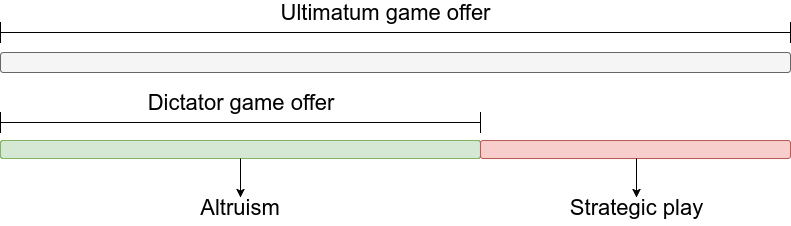
\includegraphics[width=1.\textwidth]{dictatoroffer.png}
	\label{fig:dictatorcomponent}
\end{figure}

\cite{list2007interpretation} pushback against the standard interpretation that positive offers in the dictator game reflect altruism and/or inequity aversion from the part of the proposer. For example, lower offers are seen when anonymity between proposer and responder is added, indicating that a concern about how one is seen by their peers is a driving force for the positive offers seen in the dictator game. \cite{list2004young} also find that, in the public goods game, the more anonymous decisions were amongst subjects the less the subjects opted to give in the one-shot version of the game. 

\cite{dana2006you} consider a variant of the dictator game where the proposer is given an initial endowment of \$10 and, after having made his choice, is offered the option of exiting the game with \$9. The exit option leaves the responder with nothing but ensures that he never knows that the game has been played. Even though proposers could get a higher payoff by engaging the receiver in a dictator game and not offering anything, 28\% of the proposers opted for the exit option, perhaps because they didn't want to appear unfair to the receiver were they to enter the dictator game. In their second experiment the receiver never knows whether the money offered to them comes from the proposer or from the experimenters, thus allowing the authors to determine with more clarity whether appearing to be fair is indeed a concern for proposers. They find that 9 out of 24 proposers exited, which does imply a significant minority of proposers is concerned about not appearing self-regarding to the receivers.

In \cite{dana2007exploiting} a variant of the dictator game is played. Proposers are sorted into two different treatments, the baseline and the hidden payoff treatment. In the baseline treatment, the proposer can choose one of two actions, A and B, with respective payoffs $\left(6,1\right)$ and $\left(5,5\right)$ for the proposer and responder respectively. In the hidden payoff treatment the payoff for the responder is uncertain, so proposers must choose between actions A and B where the payoffs are shown to them as $\left(6,?\right)$ and $\left(5,?\right)$. All subjects are told that the payoffs from A and B are equally likely to be either $\left(i\right)\left(6,1\right)$ and $\left(5,5\right)$, or $ \left(ii\right)\left(6,5\right)$ and $\left(5,1\right)$. The proposer can, at no cost to himself, choose to reveal the payoffs by clicking a button on the computer screen, and the responder is not made aware of that this choice has been made. The prediction is that if altruism is a better motivator for the proposer's actions the proposer will choose B in $\left(i\right)$ and A in $\left(ii\right)$. 

By comparing the proportion of proposers that chose option B in the baseline treatment with the proportion in the hidden payoff treatment that chose to reveal the payoffs the authors are able to infer whether inequity aversion is an important motivation behind the offers.

They find 14 out of 19, or 74\%, of proposers in the baseline treatment chose the more generous option B. However, in the hidden payoff treatment, 56\% did not choose to click the button to reveal the payoffs, a difference in proportion that is statistically significant. These differences imply that the appearance of being fair is an important determinant in the offers made in the dictator game and that inequity aversion does not provide a full explanation. It is possible then that at least part of the positive offers in dictator games are made not because proposers are \textit{altruists} but because they are \textit{reluctant altruists}. They want to appear to be altruists to everyone else but they would much rather keep the money to themselves.

\subsection{Gift exchange and trust games}
\subsubsection{The gift exchange game}

The gift exchange game was introduced by \cite{fehr1993} in an attempt to empirically investigate whether the notion of fairness held by agents impeded the formation of a market clearing equilibrium in labor markets, a topic first broached by \cite{akerlof1982}. 

In the \textit{gift exchange game}, two players are each assigned one of two roles: a firm or a worker. The firm offers a wage $w$ to the worker, which the worker can then reject, in which case both earn nothing, or accept, in which case the worker must now expend an effort level, $e$, of his choice. 

The standard prediction in such a setting can be discerned using a neoclassical model. Suppose the firm decides to offer the same wage to all its workers, $\omega = \bar{\omega}$. Workers have a utility function, $u(\omega,e)$, where $\omega$ is the wage rate and $e$ is the effort level they expend. The firm dictates that workers provide a minimum effort level in exchange for their wage, $e_{min}$. Workers, mindful of the firm's work rules, should choose their effort such that it maximizes:

\begin{equation}
u(\omega,e)
\end{equation}

subject to the constraints

\begin{equation}
\omega = \bar{\omega}
\end{equation}

and


\begin{equation}
e \geq e_{min}
\end{equation}


This maximization problem yields the prediction that workers will choose the lowest effort level possible, $e_{min}$. The firm, aware of this, will set $\bar{\omega}$ as low as possible in an effort to maximize profits. 

In his paper, George Akerlof is motivated to explore the effects of fairness in the formation of involuntary unemployment due to the curious results from a study of social relations among workers at a utility company in the eastern United States \citep{homans1954cash}. 

In this study, a group of women were found to be exceeding the minimum work requirements set by the firm by a considerable margin, a behavior that the neoclassical model above does not predict. Akerlof envisions this seemingly perplexing behavior as the result of the firm and the workers modelling their relationship as a "gift" exchange mediated by endogenous social norms. The workers offer a "gift" to the firm in the form of additional effort level, and in exchange the firm offers a "gift" in the form of a wage that the workers consider fair and that is in excess of what they could receive were they to leave their jobs. Thus, a labor market equilibrium is created where workers work harder because they are paid above opportunity cost. This wage level is higher than the market clearing one, ensuring that unemployment is present in equilibrium.

The gift exchange game permits us to study the level of \textit{intrinsic reciprocity} in social relations such as the one described previously. This reciprocity falls in the category of other-regarding preferences. 

Consider the following experiment from \cite{fehr1997} Subjects were assigned into one of two roles: a principal or an agent. Identities were kept anonymous, so no reputation building was possible. Principals make a job offer to the group of agents, meaning that principals stand in for employers and agents for workers.  Agents are given the option to accept or reject the offer, and in an effort to spur competition there are more agents than principals. The job offer consists of an incomplete contract, $\left ( w_b,e_n \right)$, that specifies a \textit{binding} wage level, $w_b$, and a \textit{non-binding} effort level, $e_n$. The choice of the effort level is represented by the choice of a number in which the higher the number the higher the effort is, and the higher the costs borne by the agent are. Nothing in the experiment impedes agents from choosing an effort level that is lower than the proposed effort level in the contract as there is no punishment for doing so. 

The expected behavior for both workers and firms are as noted earlier: agents will choose the lowest possible effort level and principals, knowing this, will offer the lowest possible wage level. However, if the principal believes there are sufficiently many reciprocal agents, he has an incentive to offer higher wages in an attempt to induce higher effort levels from the agents in reciprocity. Additionally, agents may induce reciprocity by the firms by offering a higher effort level than the one initially proposed.


\begin{figure}[H]
    \centering
    \caption{Relation of desired and actual effort to the rent offered to workers}
    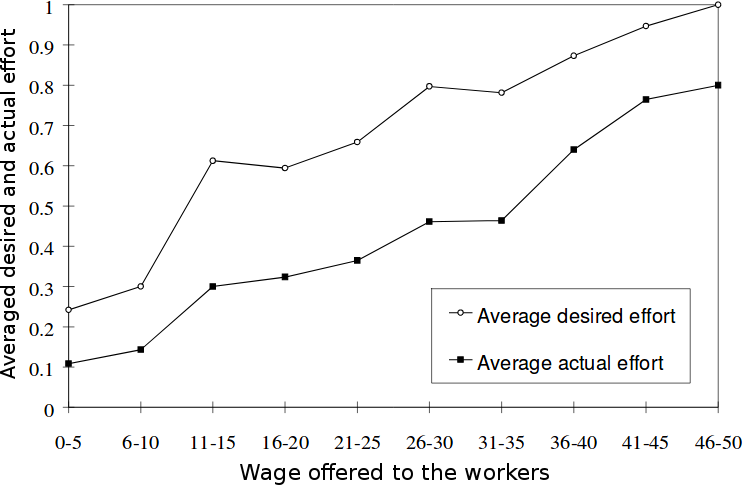
\includegraphics[width=1.\textwidth]{gift1.png}
    Source: \cite{Fehr2002}
    \label{fig:gifteffort}
\end{figure}

The experimental results are depicted in Figure \ref{fig:gifteffort}. Two conclusions follow:

\begin{enumerate}

\item Higher desired effort levels are associated with more generous offers to the workers, which suggests employers try to elicit reciprocal responses from the workers
\item \textit{On average}, the workers respond reciprocally to the employer's higher offers, though there is always a certain amount of shirking present.

\end{enumerate}

The authors further add that \textit{"there is also a substantial fraction of selfish workers who always choose the minimal effort or who rarely respond in a reciprocal manner."} The authors summarize the evidence from multiple studies to suggest that the fraction of self-regarding agents lies between 40\% to 60\%.


While we will take up the issue of the external validity of laboratory experiments in a later section, it is worthwhile to point out some of the pushback against the main conclusions of the gift exchange game that have arisen from the results gathered from the use of field studies to study reciprocity.  

\cite{Gneezy2006} hired students to a data-entry job where they would enter books into a library information system. Each student performed the task alone, and were offered \$12 for the job. In the experimental treatment, after the training phase, a portion of the students were informed they would receive \$20 per hour, with no explanation for the increase in pay. Students in the control condition were payed the previously agreed upon \$12. 

The results seemed to cast doubt over the idea that offering a wage premium is an effective measure to elicit higher worker performance. In the first 90 minutes, those workers in the treatment condition produced around 25\% more than their control peers. Although this percentage difference in effort is noteworthy, the increase in effort vanished as the experiment continued and effort levels for both treatment and control conditions where found to not be significantly different. The authors interpret their results as showing that while higher wages are reciprocated by greater effort on the part of the workers, this higher effort is not persistent and thus we need be careful to extrapolate from the single round interactions featured in the gift exchange game to how these relationships actually develop in the real world. 

A problem with \cite{Gneezy2006} is that of a small sample size, which limits their ability to detect statistical significance if the effect of a wage premium on effort is modest or small, a point mentioned by \cite{Fehr2009}. Indeed, \cite{cohn2008fairness} use a larger sample size, which allows them to have enough power to detect a statistically significant increase in effort from the increased wage, not replicating \cite{Gneezy2006}. \cite{Fehr2009} surveys the literature and concludes the positive relationship between wage and effort to be robust and well replicated. 



\subsubsection{The trust game}


The \textit{trust game} is played between an \textit{investor} and a \textit{responder}. Each player is endowed with a fixed amount of tokens, $x$. The investor must decide an amount $i \leq x$ to send to, or invest with, the responder. Before the amount chosen is delivered to the responder, the experimenter multiplies it by a multiplier $m$, meant to capture market return, and passes it on to the responder. The responder must then return an amount $r \leq mi$ back to the investor. 

If both subjects have self-regarding preferences then the responder will never send any money back to the investor. The investor, correctly anticipating the responder's behavior, will decide not to invest any amount $i$.
\\

\begin{figure}[H]
    \centering
    \caption{The trust game}
    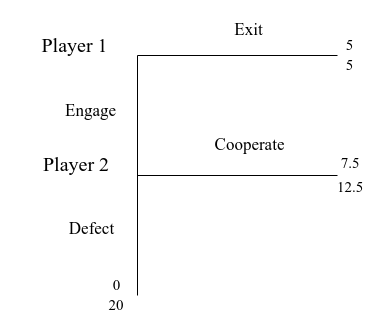
\includegraphics[width=0.65\textwidth]{trustgame.png}
    \label{fig:trustgame}
\end{figure}

We can use a concrete example to prove this prediction. Let us assume a game with two players, Player 1 and Player 2. Both are endowed with \$5. Player 1 can decide between keeping his endowment, in which case the game is ended and both players walk off with a payoff of \$5, or he may pass the entire endowment to Player 2. If the latter, the endowment is tripled by the experimenter and it is then up to Player 2 to decide whether to keep the additional \$15 for himself, or return, for example, \$7.5 to Player 1. The payoffs are, respectively, $\left( \$ 0, \$20 \right)$, and  $\left( \$ 7.5, \$12.5 \right)$

The subgame perfect Nash Equilibrium of the trust game for the self-regarding preferences model can be determined using backward induction. In the second stage of the game, Player 2 maximizes his payoff by defecting and walking off with the full amount. Predicting this, Player 1 will not send his endowment to Player 2. Thus, the predicted payoff will be $\left (\$5,\$5 \right)$, that is, both players walk out with their initial endowment, having not cooperated. Traditionally, trust game experimenters allow for both players to choose how much they intend to send to the other player, but this does not change what the subgame perfect equilibrium is. 

The share of the endowment the investor decides to invest is said to capture trust and the share sent by the responder, thrustworthiness. Both are forms of other-regarding preferences.

If both players have self-regarding preferences, then the subgame perfect equilibrium will be met. However, if both players have other-regarding preferences we should see a positive amount sent by the investor, $i>0$, and a positive amount returned by the responder, $r>0$. Figure \ref{fig:turst1} shows the distribution of offers made by both the investor and responder in a meta-analysis of 161 studies involving approximately 24,000 participants \citep{Johnson2011}.
\\



\begin{figure}[H]
    \centering
    \caption{Distribution of percentages sent by investors (left) and responders (right).}
    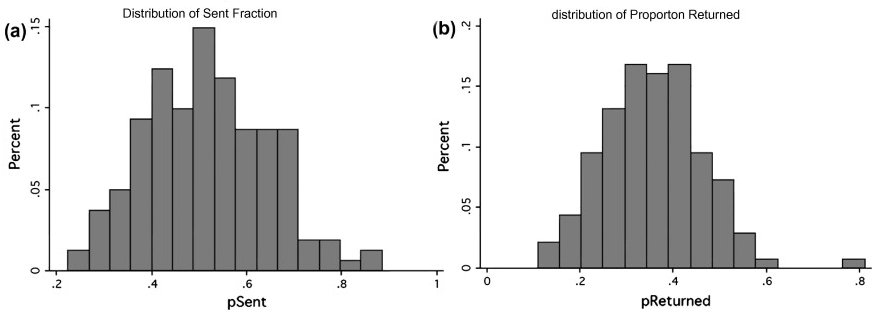
\includegraphics[width=1\textwidth]{figure_trust1.png}
    Source: \cite{Johnson2011}
    \label{fig:turst1}
\end{figure}


The meta-analysis found that the mean offer made by the investor across all studies is .502, around half of the initial endowment, while the mean amount returned by the responder is .372. Due to aggregation of multiple experiments from multiple parts of the world the authors were able to study the differences in how people from around the world play the trust game. They find Africa sends and receives the lowest amount of all continents, with North America and Europe featuring the highest amounts both sent and received. They find further that older people send larger amounts, students send significantly lower amounts than non-students, and that amounts sent are larger if the subject believes he is playing with another human player. 
%\subsection{Public goods games}
%\subsubsection{Public goods game without punishments}
%
%
%Let's assume a game with $n > 2$ players, each with an initial endowment of $y$ monetary units. Each player must simultaneously decide on their respective contributions, $g_i \geq 0$ to a public good. The total monetary contribution to the public good is given by $G = \sum^n_{i=1} g_i$. The monetary payoff of each individual is given by:
%
%\begin{equation}\label{publicgoods}
%    m_i = y-g_i +rG; \frac{1}{n}<r<1
%\end{equation}
%
%where $r$ is meant to represent the return, or benefit, to an individual from one unit of the public good, i.e., we can define $r$ as the marginal per capita return (MPCR).
%
%If all players in the game have self-regarding preferences all their actions will involve \textit{free riding}, i.e, $g_i^* = 0$. To see that this is so let the vector of the contributions made by other players be $\pmb{g}_{-i}^* = \pmb{0}$. Using \eqref{publicgoods}, we see that 
%
%\begin{equation}
%\frac{\partial m_i}{\partial g_i} = r - 1 < 0
%\end{equation}
%
%which implies that the that the individual will be worse off by contributing to the public good, hence the optimal contribution is $g_i^* = 0$.
%
%To see that the social optimum is characterized by all players contributing their full endowment $y$, note that, we can find the social optimum by solving 
%
%\begin{equation}
%\frac{\partial \sum m_i}{\partial g_i} = \frac{\partial \left( ny-G+rnG\right)}{\partial g_i} = rn-1>0 
%\end{equation}
%
%which implies that the total monetary payoff is maximized when players contribute as much as they possibly can, which in the context of this game is their full endowment $y$.
%
%\subsubsection{Public goods game with punishments}
%
%There's two stages to the public goods game with punishments. In the first stage the players play the public goods game without punishments. In the second stage, after the individual contributions to the public good are made publicly available, each player chooses a punishment vector $\bm{p}_i = \left( p_{i1},...,p_{in}\right)$ where $p_{ij}$ is the punishment inflicted by player $i$ on player $j$ at a cost of $c$ per unit of punishment and $0<c<1$. 
%
%As with the game without punishments, the equilibrium for individuals with self-regarding preferences is one where all players free-ride. To see this, lets assume a vector of contributions made by$n$ players in the first round $\left(g_1,g_2,...,g_n\right)$. Independently of the vector of punishments from other players, $\pmb{p_{-i}}$, the payoff of player $i$ is maximized when $\pmb{p}_i = \pmb{0}$. Hence, it is a dominant strategy for each player not to engage in any sort of punishment, which reduces the game to the public goods game without punishments where, as saw, the Nash Equilibrium was free-riding by all players.
%
%\subsubsection{Empirical evidence}
%
%The evidence from one shot public goods games without punishments show little support to the idea that agents have self-regarding preferences and thus play according to the predicted equilibrium [CITE DAWES THALER 1988]. While not every subject contributes to the public good, on average, those that do contribute about 40 to 60\% of their endowment. This result does not depend on whether subjects have played the game before, on the size of the group playing, or the stakes in the game, though average contributions do lower when stakes are higher [CITE MARWELL AMES 1981)].
%
%This general line of results is however put into question when subjects play a public goods games without punishments multiple times. What is usually seen in these cases is that in the first round the results are in line with what is observed in the one shot version of the game. However, in the following rounds, cooperation drops sharply and towards the last round the contributions for most subjects are close to zero, as predicted by the model with self-regarding preferences. [FEHR SMIDTH 1999] summarize the results from multiple repeated public goods games without punishments and say that approximately 73\% of all subjects choose to free-ride, with a significant portion of the remaining ones playing very close to the equilibrium strategy. They add that, in light of these facts, "it seems fair to say that the standard model 'approximates' the choices of a big majority of subjects rather well."
%
%A very different picture emerges when we consider the public goods game with punishments. As we've seen, the equilibrium strategy in this version of the game is the same as in the one without punishments. Subjects are expected to free ride. However, when the possibility of punishing other players is put into the design of the experiment, close to 83\% of players choose to cooperate \textit{fully}. That is, when punishments are added, a majority of the players contribute their whole endowment towards the public good [FEHR GACHTER 2000]
%\\
%
%[FIGURE]
%\\
%

\section{On the Validity of Using Experiments in Economics}

\begin{quote}{\cite{Samuelson1985}}
"One possible way of figuring out economic laws ... is by controlled experiments... Economists [unfortunately]... cannot perform the controlled experiments of chemists or biologists because they cannot easily control other important factors. Like astronomers or meteorologists, they generally must be content largely to observe"
\end{quote}

Laboratory experiments are a widely used tool in the physical and life sciences. In contrast, the social sciences have traditionally been considered nonexperimental, that is, the data upon which social scientists base their theories are collected not through experimentation, but observation. This is due to the obvious constraints of this class of scientific disciplines (e.g. historians are not able to recreate in a lab the Napoleonic Wars). This is not to say the social sciences have not or do not use laboratory experiments when it is feasible to do so. Psychology, for instance, has used laboratory experiments, or the experimental method more broadly, successfully for more than two centuries now (e.g. \cite{Ebbinghaus1885}). In economics, however, the use of laboratory experiments is a recent development. 

Although there was some proto-experimental work done in the 1930s on the topic of consumer demand theory \citep{Moscati2007}, it is generally agreed that, as an institutional and intellectual programme, experimental economics took form in the late 1940s following the publication of John von Neumann and Oskar Morgenstern seminal \textit{Theory of Games and Economic Behavior} in 1944 \citep{Guala2008}. Since then, the growth of published papers using laboratory experiments has been remarkable. 

In three of the most prestigious economics journals --- \textit{American Economic Review, Econometrica}, and \textit{Quarterly Journal of Economics} --- the fraction of experimental papers published in proportion to all published papers was between $0.84\%$ and $1.58\%$ in the 1980s, jumping to $3.8\%$ and $4.15\%$ between 2000 and 2008 \citep{Falk2009}. The first specialty journal, aptly named \textit{Experimental Economics}, was founded in 1998. Moreover, $6\%$ of the Nobel economics prizes awarded since 1969 have been to economists who can be described as working in experimental economics, including heavyweights such as Elinor Ostrom, Daniel Kahneman, and, more recently, Richard Thaler. The rise in prominence of experimental economics has been such that, despite the above quote from Samuelson and Nordhaus, in the 1992 revision of their famous textbook they saw the need to further add that experimental economics is "an exciting new development"\citep[p.~5]{Samuelson1992}.

\begin{figure}[H]
	\centering
	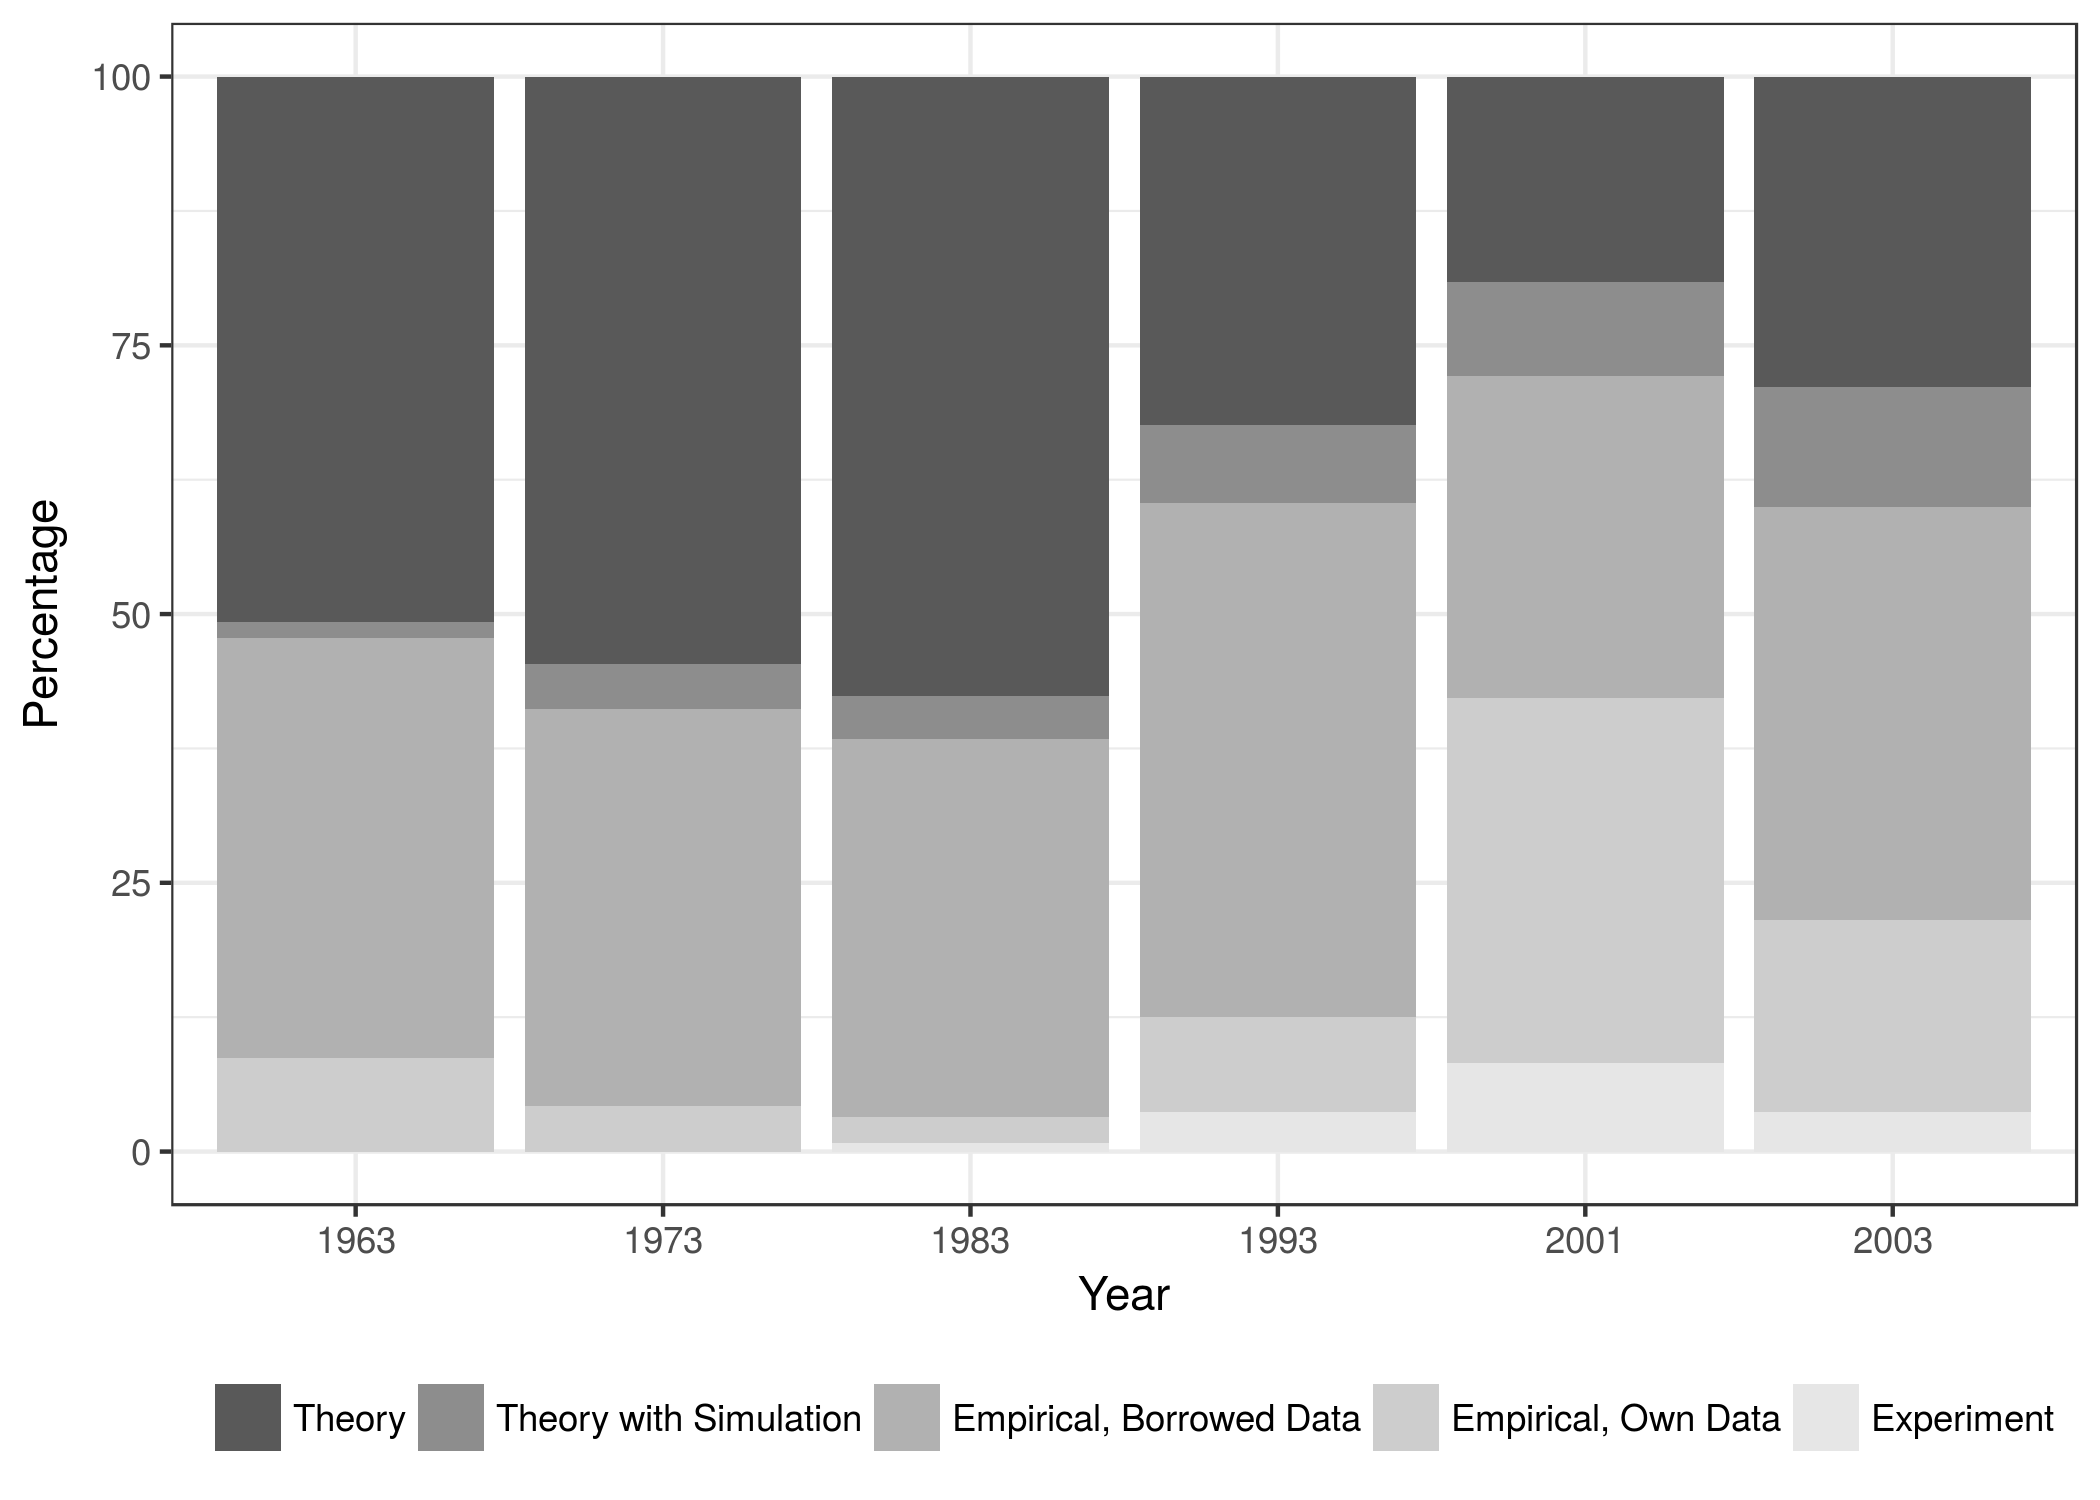
\includegraphics[width=1.\textwidth]{proportion.png}
	\caption{Methodology of articles in top economics journals, as percent of total. Source: \citep{mearsheimer2013leaving}}
	\label{fig:proportion}
\end{figure}


There is however an elephant in the room. Despite the evident growth in the use of laboratory experiments in Economics, there have been challenges regarding whether the result coming out from these experiments allow researchers to say anything about economic behavior outside the lab. The issue of external validity, the ability of experiments to provide findings that are likely to allow for reliable inferences outside the laboratory, is a pernicious problem for the social sciences that does not exist to the same extent in the physical sciences.

By way of illumination, a Physics student performing a careful experiment to determine the value for Earth's gravity need not concern himself as to whether his results will generalize to outside the lab. The same is not necessarily true in the social sciences, in general, and for most of the experiments we have surveyed above, in particular. While it does seem that subjects offer around 20\% of their endowment in the dictator game, we do not regularly see strangers in the streets spontaneously offering a fifth of the contents in their wallets to strangers passing by. 

If we are to use the extensive evidence surveyed previously to argue for the existence of other-regarding preferences we must first establish that it offers us reliable evidence that extends beyond the artificial conditions of the laboratory. Indeed, it is this artificiality that, while imbuing laboratory experiments with their unique methodological strength, also gives it the weakness that has been an influential source of skepticism about their use as a tool in the economist's toolbag.

Laboratory experiments are often contrasted with field experiments. In the debate between the two, field experiments are often touted as possessing more 'realistic' conditions,  even if they are perhaps less tightly controlled. 

\cite{List2006} provides an interesting example of this idea. In his paper, a gift exchange game is played where buyers make price offers to sellers and, in return, sellers select the quality of the good they will exchange with the buyer. The experiment was run in a standard laboratory setting and used experienced sports-card traders as subjects. The results mirrored the typical findings for this type of game: in the presence of higher offered prices, sellers tended to offer higher quality goods in return, even though they were not obligated to do so by the rules of the experiment. Thus this laboratory experiment points toward the existence of other-regarding preferences in the gift exchange game. 

The experiment was then carried out by making a single change in which the goods exchanged where actual baseball cards whose market value was influenced by differences in their physical condition that experienced card sellers are more likely to detect than unexperienced sellers. In this experiment, other-regarding preferences were also observed. Higher quality cards were offered to buyers who offered higher prices.

The two experiments are therefore concordant in their conclusion of the existence of other-regarding preferences. However, List did not stop there. He wanted to know whether his results would also be observed in the card sellers natural environment, a sports-card show. Dealers in this field study were unaware that their behavior was being observed and studied. Confederates were instructed to approach sellers and offer different prices in return for sports-cards of varying quality, mirroring the methodology of the previous experiments. 

In this field study, where the dealers did not believe that the consumers could grade the cards appropriately or there was little possibility of future interaction, little statistical relationship between price and quality was observed. Only when there was concern for one's reputational standing, when sellers expected future interactions to happen or buyers could verify the quality of the cards by using a third-party, was high offered price met with high quality offered. Thus, the other-regarding preferences routinely observed in the lab were attenuated or not observed in the field condition.\footnote{\cite{camerer2011promise} provides a critical reply to \cite{List2006} and reanalyzes the data with different statistical techniques. He notes that "...the conclusion that the lab and field show different reciprocity is suggestive but is just not robustly significant."}

The dichotomy of results between the laboratory and field conditions should certainly make us pause before claiming with certainty that other-regarding preferences matter in an economic context. It is tempting to think that field experiments reflect a more realistic condition and should thus be held in higher regard when making inferences about the inexistence of other-regarding preferences. Thus, that card dealers do not seem to match quality with price in a sports-card show seems to suggest that we should not change our priors with regards to the existence of other-regarding preferences. It is however worth thinking more deeply about this notion that field studies offer us a more realistic picture than laboratory experiments.

\cite{camerer2011promise} makes the helpful distinction between the \textit{policy view} and the \textit{scientific view}. In the policy view, the generalizability of experimental findings to the outside world, that is, their \textit{external validity}, is of paramount importance. This is because in choosing what policy to apply, evidence that has been collected in the same domain as the policy has obvious advantages in the inferences one can draw from it with respect to the effects of policy in question. Field experiments should be given more weight in this view than laboratory experiments do. For the scientific view, however, both laboratory and field studies constitute  ways to enhance our understanding of human behavior and should therefore hold equal weight in the inference process. Provided the evidence was properly gathered and is valid and contextually relevant, there is no hierarchical relationship between the two methodologies. Both constitute tools to be used in the accumulation of knowledge. As Camerer puts it: "in this view, since the goal is to understand general principles, whether the 'lab generalizes to the field' ... is distracting, difficult to know ..., and is no more useful than asking whether 'the field generalizes to the lab'."

To illustrate this point, consider the following formalization from \cite{Falk2009}. Suppose a variable of interest $Y$ can be fully explained by the variables $X_1,...,X_N$ and that the functional relationship between them is given by $Y=f\left(X_1,...,X_N\right)$, known as the all-causes model. Suppose we are interested in examining the causal effect of $X_1$ on $Y$, which requires us to hold all other variables $\hat{X} = \left(X_2,X_3,.., X_N\right)$ fixed.

In a laboratory experiment the researcher estimates a model of the form $Y=f\left(X_1,X^L\right)$ where $X^L \neq \hat{X}$. Following the same logic, in a field experiment one estimates a model of the form $Y=f\left(X_1,X^{F_1}\right)$ where $X^{F_1} \neq \hat{X}$ and typically $X^{F_1} \neq X^L$. The claim is usually made that $f\left(X_1,X^L\right)$ does not satisfy external validity but $f\left(X_1,X^{F_1}\right)$ does.

We can write the field study in \cite{List2006} as $Y=f\left(X_1,X^{F_1}\right)$ where $Y$ is the quality of the cards, $X_1$ is the price offered, and $X^{F_1}$ are the remaining variables. Suppose we were to repeat that same experiment using a different subject pool, possibly stamp collectors. This gives rise to yet another estimated relation $Y=f\left(X_1,X^{F_2}\right)$ where $X^{F_2}$ reflects the set of variables and characteristics in this new experiment, including the new subject pool. How are we to adjudicate between $f(X_1,X^L)$ and $f(X_1,X^{F_1})$ if we want to predict the causal relationship between $X_1$ and $Y$ in the new relation $Y=f\left(X_1,X^{F_2}\right)$?

One might be tempted to reply that the field experiment should hold more weight than the laboratory experiment in this particular inference since the new situation also involves a field experiment. There is not, however, an explicit reason for why this should be so. While both situations are field experiments, there is no a priori reason to expect the behavior from sports-card dealers to generalize toward that of stamp collectors. As \cite{camerer2011promise} puts it (using different notation), "if the litmus test of 'external validity' is accurate extrapolation to $X^{F_2}$, is the lab $X^L$ necessarily less externally valid than the field setting $X^{F_1}$? How should this even be judged?"

It is best then, under the scientific view, to treat laboratory and field data as complementary. Both have their strengths, and the usefulness of one versus the other is ultimately a matter of the underlying research question. Laboratory experiments, due to their tight control, are more prone to be replicable whereas in field experiments replicability can be challenging and is more often than not impossible. The smaller cost of laboratory experiments, as well as the easiness of archiving and reproducing instructions, software, recruiting protocols, databases, and statistical tools, also make laboratory experiments easier to replicate. 

The two methods differ in what variables $\hat{X}$ they are able to provide a larger variation for. Laboratory experiments can explore the parameter space for values that can be hard or rare to find in the field. For example, in \cite{andersen2011stakes} the authors raise the stakes in the ultimatum game by a factor of 1,000 such that the highest stakes in play equal 16,000 hours of work, an amount that would be nigh impossible to find in the field. Field experiments do a better job at collecting evidence for different subject pools with different demographics and social characteristics, as we saw in the multidisciplinary work of \cite{henrich2005economic} who employed the ultimatum, dictator, and public goods game in 15 small-scale societies. 

Having argued for the usefulness of laboratory experiments, there still remain some concerns that need be addressed before we can be safe in using the experimental evidence to argue for the existence of other-regarding preferences. While we have seen that there is no a priori reason for laboratory experiments to not be used in the making of inferences about economic behavior in lieu of field experiments, this is only so if laboratory experiments are a valid tool for the study of this particular subject. That is, while by themselves laboratory experiments are a valid tool in the economist's toolbox, there might be flaws in the experimental process that invalid the use of the results gathered to infer the existence of other-regarding preferences. A powerful critique of the experimental method is offered in \cite{levitt2007laboratory} where the authors raise legitimate concerns that put into question the external validity of the observed results.

By the order in which these objections will be tackled, they are:

\begin{enumerate}
	\item There is unprecedented experimental scrutiny in laboratory experiments. This may give rise to \textit{experimenter demand effects} where subjects, perceiving that they are being observed by the experimenter, may behave in ways that they believe the experimenters desire, or may also behave in ways that end up not revealing their true preferences, e.g., being observed may lead to more prosocial behavior than the subject actually desires. 
	\item Human behavior is context-dependent and it is not clear that experiments can either capture or control this.
	\item There is the possibility of self-selection bias where experiments might be being run with an homogeneous sample of students who might be more prosocial, more educated, and have a higher need for approval than the average human population.
\end{enumerate}

Levitt and List additionally question the common use of small stakes in laboratory experiments arguing that it might not capture the richness of human behavior. We choose not to deal with this objection because the previous section already dealt with the effects of varying stake size in the experiments. Indeed, the issue of stake size has long been a topic of interest in behavioral economics \citep{camerer1999effects} and is no longer a novel nor potent objection.\footnote{As Colin Camerer writes in his 2003 textbook, five years before Levitt and List's paper: "If I had a dollar for every time an economist claimed that raising the stakes would drive ultimatum behavior towards self-interest, I'd have a private jet on standby all day \citep[p.~60]{camerer2011behavioral}."}
\\

\textbf{Experimenter demand and audience effects}
\\

Subjects in laboratory experiments know that their behavior is being recorded and will be under intense scrutiny. This intense obtrusiveness might lead to subjects matching their behavior with what they perceive to be the experimenter's desired behavior (\textit{experimenter demand effect}), or may lead subjects to behave in more prosocial ways because they believe that self-regarding behavior may be frowned upon by the experimenter (\textit{audience effect}).

Let us assume for a moment that subjects hold an accurate view of what the experimenters expect and favor a particular outcome, which is not obvious and is something that experimenters are aware of when designing experimental procedures and thus work to circumvent. For there to be a demand effect it is necessary that the subject be willing to sacrifice his earnings by behaving in the way that the experimenter desires. Even if the subject is willing to do so, that willingness is but a component of his overall preference bundle, meaning that it should be possible to devise a situation that stresses his initial desire and makes him more reluctant to sacrifice his earnings. That increasing the stakes involved in the experiments typically has little effect suggests that demand effects are not a strong concern.

This still leaves us with the possibility that the intense experimental scrutiny leads to subjects behaving more prosocially. \cite{barmettler2012big} employ a novel experimental procedure that allows the manipulation of experimenter-subject anonymity and employ it in three experimental games: the ultimatum, the dictator, and the trust game. In none of these, for any player in any role, is there a statistical significant difference in the choices made between the treatment condition where anonymity between subject and experimenter is maintained and the one where it isn't.

Experimenter demand and audience effects do not seem to be strong objections against the experimental evidence. Indeed, if experimental scrutiny made such a noticeable effect on the emergence of other-regarding preferences that would itself be evidence for the existence of other-regarding preferences for we are regularly being directly observed in many of our real-world interactions. More distopically, if scrutiny was a powerful enough force to flip a person's switch towards behaving more prosocially, it is likely we would be seeing intense institutional efforts to promote that scrutiny.
\\

\textbf{Context dependence}
\\

Human behavior is embedded in a rich, complex, and tangled web of social norms, frames, and the lessons learned from past experience. Levitt and List argue that different experimental procedures, such as writing the instructions the subjects read in different ways, may lead to differing results. Defection rates in the prisoner dilemma game vary depending on whether subjects are playing a "Community" or "Wall Street" game \citep{ward1997naive}, framing the allocation of funds in a public goods game as a "contribution" or "allocation" matters, as does whether the game is framed as a positive externality or a negative one \citep{Andreoni1995}.

However, even though Levitt and List make a persuasive case for the importance of the context, they also argue that this context is "is not completely controlled by the experimenter." This collides with their previous argument because if it is possible to elicit different results by varying some of the experiment's parameters then it follows that it is also possible to control and account for that context. Indeed, that variation is highly desirable in the scientific view since it allows for the accumulation of knowledge about the boundary conditions of human behavior. Thus the very idea that experimental context might influence the results is an argument for more experiments to be run.

Moreover, to the extent that there is a subset of context that is not liable of being captured by any methodological variation, then it is also unlikely that uncaptured context is possible to control for in a field experiment. The problem of uncontrolled variables that cannot be measured and controlled for is not a problem of laboratory experiments per se, for field studies also run into it, but is instead a problem that every empiricist must wrestle and contend with. 
\\

\textbf{Self-selection bias}
\\

The empirical evidence we have surveyed is largely based on laboratory experiments using self-selected students. This homogeneous sample might constitute a problem if students are found to behave in systematically different ways than the rest of the population. If the students who self-select into experiments behave more prosocially then the results provide a biased estimate of the extent to which there are other-regarding preferences in the population.

\cite{falk2013lab} provide an interesting study of this question where they are able to distinguish whether students who self-select into laboratory experiments are any different from those students who don't, as well as whether these have different social preferences from the rest of the population. 

They analyze the decisions of a sample of 16,666 undergraduates at the University of Zurich for which they know who participated in experiments and how many times. To measure the extent of their prosocial inclinations they use data collected from a naturally occurring repeated decision where each student must decide whether or not he or she wants to contribute a predeterminate amount to two social funds which provide charitable services. The authors conclude that participating students do not have different social preferences than their nonparticipating colleagues. If there is a bias then it is because students are different from everyone else.

To see if such a difference exists the authors employ two identical trust games using distinct subject pools so that the only difference in prosocial behavior comes from differences between the two subject pools employed and not changes in experimental design. One group was recruited from the student pool at the University of Zurich and the other from a representative sample of the population of the city of Zurich. In total 1,296 participants were recruited (295 students and 1,001 from the general population) 

They find that the non-student subject pool behaves more prosocially than the student subject pool which implies that by regularly employing students in their experiments researchers might be downwardly biasing their inferences about the existence of other-regarding preferences, i.e., to the extent that this is an issue is more one of magnitude than direction. The finding that students exhibit less prosocial behavior than the rest of the population is consistent with a range of other evidence, e.g., CEOs tend to be more prosocial than students \citep{fehr2004hidden}.

Indeed, concerns about the homogeneity of the subject pools used in laboratory experiments being problematic has been dealt with powerfully with the experiments performed by \cite{henrich2005economic}. Even though they report wide variation in the extent to which people in different societies have other-regarding preferences, the fact that none of the societies studied confirmed the self-regarding predictions implies that other-regarding preferences may well be a general feature of human nature. 


\section{Moddeling Other-Regarding Preferences}

The evidence surveyed previously establishes that agents often have preoccupations not only about what happens to themselves but also with what happens to other people. Economic models often do not include these social preferences in their structure, possibly limiting the set of behaviors they are able to explore. At worst, by not taking into account the existence of other-regarding preferences these models may reach incorrect conclusions about the economic behavior of agents.

There is thus the need for a theoretical model that takes into account the empirical findings on other-regarding preferences. The Fehr-Schmidt model of inequity aversion developed in \cite{Fehr1999} is a proposal for such a model. A description of this model and an application to the ultimatum game follows.

\subsection{The Fehr-Schmidt Model of Inequity Aversion}

Consider $n$ individuals, each with a respective monetary payoff $y_1,y_2,...,y_n$. The payoffs of all individuals but the individual $i$ is denoted by the vector $\vec{y}_{-i}$. For any $i$, the Fehr-Schmidt utility function, henceforth FS utility function, is defined as:

\begin{equation}
\begin{split}
	U_i\left(y_i,\vec{y}_{-i};\alpha_i,\beta_i\right) = y_i &- \frac{\alpha_i}{n-1} \sum_{j\neq i} \max \left \{ y_j - y_i,0 \right \}\\
	& - \frac{\beta_i}{n-1} \sum_{j\neq i} \max \left \{ y_i - y_j,0 \right \}
\end{split}
\end{equation}


\noindent
where $\alpha_i \geq 0$ and $0 \leq \beta_i <1$. It is easy to see that the FS utility function describes an individual with self-regarding preferences if $\alpha_i = \beta_i = 0$, in which case $U_i\left(y_i,\vec{y}_{-i};\alpha_i,\beta_i\right) \rightarrow U_i\left(y_i\right)$.

The FS utility function models the individual as comparing his situation with the situation of the individuals around him. That is, the individual exhibits self-centered inequity aversion, where some people are better off than him and he his better off than other people. This is captured by the second and third terms in the function, respectively.

The second term in the FS utility function measures the utility loss from disadvantageous inequality, more coloquially called envy, while the third term measures the loss from advantageous inequality, or altruism. It is assumed that $\alpha_i \geq \beta_i$. This means that, for the same magnitude, an individual loses more utility from another individual being better of than him than in the contrary situation. Envy is a more psychologically salient condition than altruism.

While there is no upper bound on $\alpha_i$, it is assumed that $\beta_i <1$. The reasoning for this upper bound is that when an individual with $\beta_i \geq 1$ reduces his advantage over other individuals he is increasing his utility by more than he is reducing his advantage. This seems implausible as it would require extremely high levels of altruism from the individual. \cite{Eckel2010} report the magnitudes of $\alpha$ and $\beta$ from various studies. The evidence indeed suggests that for most individuals $\beta <1$ and $\beta <\alpha$.

%For $\alpha$ no such upper bound exists because the individual, in the case where he compares his situation with only one other individual, for example, is prepared to give up one monetary unit if the corresponding decrease for the remaining individual is $\left(1+\alpha_i\right)/\alpha_i$ units. 


We will now see how the Fehr-Schmidt model can be used to understand the behavior seen in the ultimatum game that was previously unexplainable using models with just self-regarding preferences.

\subsubsection{The ultimatum Game}

A proposer and a responder play the ultimatum game. They are, respectively, Player 1 and Player 2. Of the full endowment researchers award to Player 1, the share of it that is proposed is denoted by $s$.

\begin{lemma}
	The responder accepts all offers $s \geq 0.5$. There is a critical share, $s_c < 0.5$ such that the responder rejects all offers below it and accepts all offers $s \geq s_c$.
\end{lemma}

\begin{proof}
	If $s>0.5$, taking into account the FS utility function for the case with only 2 players, we have the following for the responder:
	
	\begin{equation}
		U_2 = s - \beta_2 \left[s - \left(1-s\right)\right]
	\end{equation}

	\noindent	
	which is positive because $\beta \in \left[0,1\right)$, hence the responder will accept.
	
	Now suppose $s<0.5$. In this case we have
	
	\begin{equation}
		U_2 = s - \alpha_2 \left[\left(1-s\right) - s  \right] = s(1+2\alpha_2)-\alpha_2
	\end{equation}
	
	For this to be positive we need $s$ such that 
	
	\begin{equation*}
		s \geq \frac{\alpha_2}{1+2\alpha_2}
	\end{equation*}
	
	Taking $\alpha \rightarrow \infty$ reveals that the critical threshold, $s_c$, is 0.5.
	
\end{proof}

\begin{prop}
	The equilibrium share offered by the proposer is given by:
	
	\begin{equation}
		s^* =\left\{\begin{matrix}
		s_c & \text{if} & \beta_1 <0.5\\ 
		0.5 & \text{if}&\beta_1 >0.5\\ 
		s_ \in \left[s_c,0.5 \right] & \text{if}&\beta_1 =0.5
		\end{matrix}\right.
	\end{equation}	
\end{prop}

From the previous lemma we know that the responder will accept any share $s_c \leq s \leq 0.5$.  Let us consider such a share. From the FS utility function we have, for the proposer, $U_1 = \left(1-s\right) - \beta_1 \left[\left(1-s\right)-s\right]$. Taking the first derivative with respect to $s$ leaves us with $2\beta_1 -1$. Thus, if $\beta_1 < 0.5$, we have $\frac{\partial U_1}{\partial s}<0$ so the proposer should offer the minimum possible that the responder will accept, i.e., $s_c$.

If $\beta_1 = 0.5$ we have $\frac{\partial U_1}{\partial s}=0$ so any feasible share between $s_c$ and 0.5 may be offered and will be accepted.

For values of $\beta_1$ higher than 0.5, $\frac{\partial U_1}{\partial s}>0$, so we have $s^* = 0.5$.

Given what we know about the results usually observed from playing the ultimatum game, we can see that the Fehr-Schmidt model matches the experimental results reasonably well. Fehr and Schmidt note that their model "yields too extreme predictions in ... the dictator game", where proposers only offer high offers $\left(s = 0.5\right)$ or very low offers $\left(s = 0\right)$, a prediction rejected by the data. 

They note that their model can easily be modified so that the assumption that inequity aversion is linear can be dropped and substituted by a utility function that is concave in the amount of advantageous inequality. With this new assumption the results of the dictator game can also be accommodated. 

\section{Contract Design Under Other-Regarding Preferences}

The results from the gift exchange game surveyed previously indicate that reciprocity influences the relationship between principal and worker in that the principal can elicit more effort from the worker by offering a higher wage even though there are no guarantees that the worker will reciprocate by exerting a higher effort. This leads us to question how these deviations from the self-regarding model influence how best to structure the incentives that mediate the relationship between the two parties. 

In this section we will apply what we have learned about other-regarding preferences to understand how they affect the optimal choice between competing types of contracts under the existence of moral hazard. More colloquially, we are interested in knowing whether it is best for the principal to reach for the carrot rather than the stick.

Consider a principal who contracts an agent to work for him. The agent can expend effort $e \in \left[\ubar{e},\bar{e}\right]$ at a cost $c\left(e\right)$ such that ${c}'>0$ and ${c}''>0$, where $c(e)$ denotes the effort cost function. The principal wants the agent to expend $e_{min}$, which he introduces in the contract as the contracted effort level. However, $e_{min}$ is non-binding since the agent's effort is not verifiable. Because the principal might want to provide evidence to a third party in the case where the worker is expending less effort than the contracted one the principal might invest in a verification technology that costs $k$. This technology is able to provide evidence of shirking with a probability $p\in \left(0,1\right)$ which the principal can then use to impose a fine $f$ on the agent.

In \cite{fehr2007fairness} a cohort of individuals are randomly selected into the roles of principal and agent and are then matched into principal-agent pairs. The game is played for 10 periods where in each one a new pair is created so that no agent interacts more than once with the same principal. In the first stage of the game the principal chooses the type of contract and whether to invest in a verification technology; he proceeds to make an offer to the agent he is matched with. In the second stage the agent decides whether to accept the contract and, if he does, how much effort to expend. In the third and final stage, if the principal has invested in the verification technology, evidence of the agent's effort level is obtained with probability $p$ and the terms of the contract are enforced.

The three types of contract the principal has at his disposal to offer are:

\begin{itemize}
	\item \textbf{Incentive contract}: The contract specifies the wage $w$, the contracted effort level $e_c$, and the maximum fine $\bar{f}$ to be imposed on the agent if evidence of shirking is discovered. It is assumed the principal has invested in the verification technology.
	\item \textbf{Trust contract}: The contract specifies the wage $w$ and the contracted effort level $e_c$ but there is no investment in the verification technology. Therefore, $e_c$ is non-verifiable and $w$ is not contingent on the actual effort of the agent.
	\item \textbf{Bonus contract}: This contract is similar to the trust contract except where if the agent expends an effort level superior to $e_c$ the principal might choose to reward the agent by offering a bonus $b$, which is not enforceable.
\end{itemize}

An analysis of what type of contract the principal would find preferable to offer under the assumption of self-regarding agents and principals is similar to the one made for the gift exchange game. Given the non-enforceability of $e_c$ in both the trust and bonus contracts, and the added non-enforceability of $b$ in the bonus contract, it is trivial to conclude that self-regarding agents will exert the lowest possible effort level. 

However, the principal is able to induce a positive effort level from the agent if the verification technology is potent enough so that $p\bar{f} \geq c(e^*) - c(\ubar{e})$. Therefore, under the assumption of self-regarding preferences, the principal will choose the incentive contract over the other two available alternatives: the trust and bonus contracts. This is a testable prediction.

\cite{fehr2007fairness} features two different experiments, one where principals can choose between a trust and an incentive contract and another where principals choose between a bonus and an incentive contract. In the trust-incentive experiment the self-regarding preferences are largely confirmed. Most principals choose to offer agents an incentive contract and their share, over the 10 rounds played, increases over time. While there is experimentation on the part of most principals by offering a trust contract at least once, the differences in payoffs from both contracts were such that principals preferred the incentive contract. Once principals learned how to create an appropriate incentive contract with the right mix of $w$, $e_c$, and $f$, they made up the large majority of contracts offered.


\begin{figure}[H]
	\centering
	\caption{Share of bonus and incentive contracts in the bonus-incentive experiment}	
	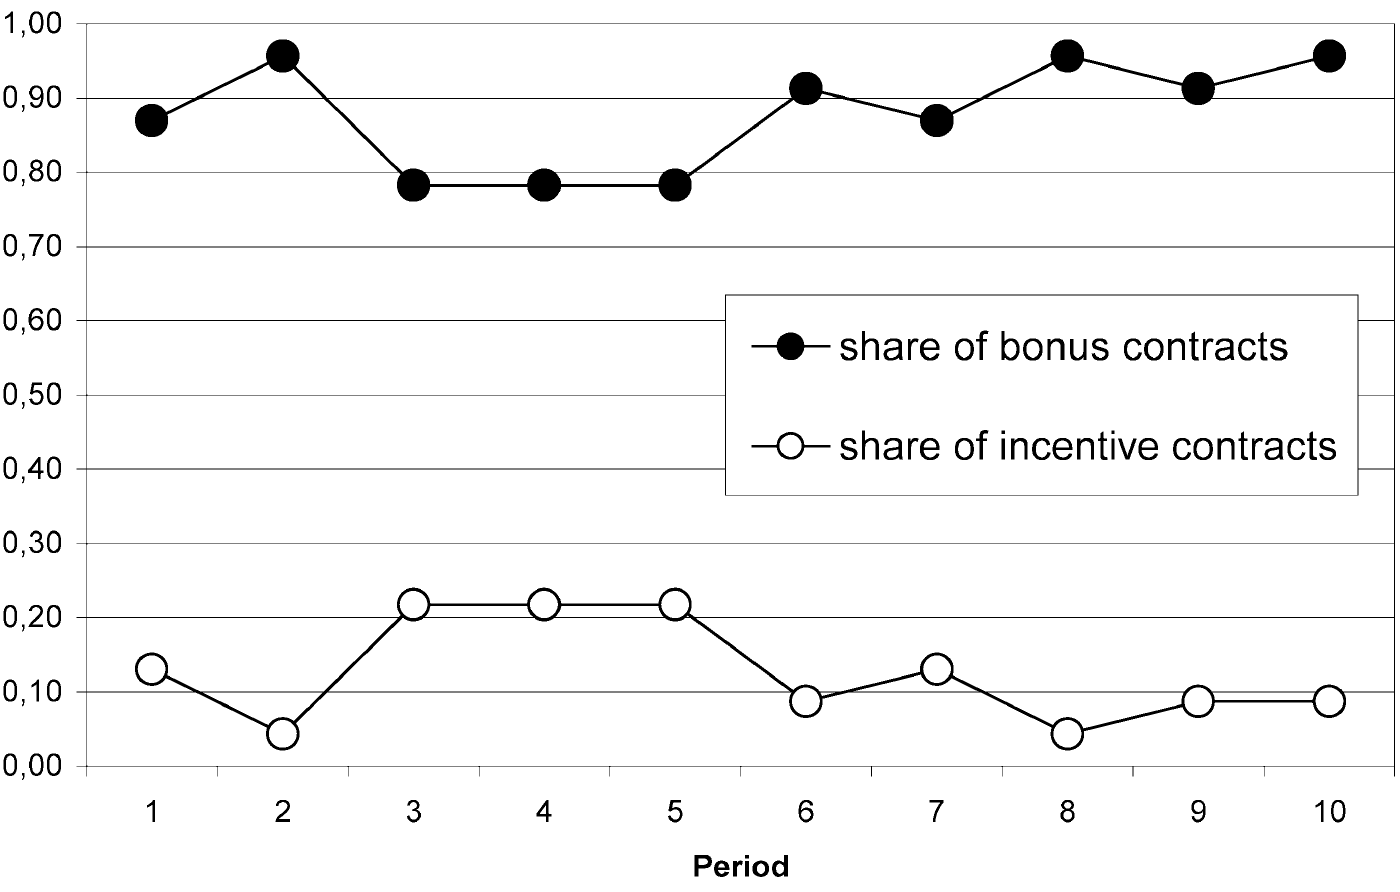
\includegraphics[width=1.\textwidth]{bonusincentive.png}
	 Source: \cite{fehr2007fairness}
	\label{fig:bonusincentive}
\end{figure}


It is in the bonus-incentive experiment that deviations from the self-regarding prediction are observed. Recall that the bonus $b$ in the bonus contract is non-enforceable. If the principal, in his self-regarding rationale, decides not to offer a bonus, then the bonus contract becomes a trust one. Since agents are aware that the bonus is non-binding and therefore not likely to be realized, they should equate the bonus contract with the trust one and act accordingly. This would lead us to predict that in the bonus-incentive experiment we should observe results similar to those from the trust-incentive one. This prediction is, however, not confirmed by the experimental results.



The overwhelming majority of contracts in the bonus-incentive experiment are bonus contracts, with the incentive contract seldom being offered. This choice is driven by the ability of bonus contracts to elicit a higher effort level from the agents which increases the payoff the principals get in comparison with the possible payoffs from the other contracts. Part of this larger surplus is then allocated by the principals as a bonus to the agents. The average income gained by agents in the bonus contract is approximately 23\% higher than the one earned in the incentive contract. It turns out therefore that that the use of a bonus contract is beneficial to both parties.

Since the self-regarding model does not explain this set of choices, we will suppose an alternative where both the agent and the principal have other-regarding preferences of the Fehr-Schmidt form. This analysis follows closely \cite{dhami2016foundations}. 

For simplicity we will assume that the agent's output, $\nu(e)$, is equal to $e$ while the effort cost function is $c(e)=\frac{1}{2}e^2$ where $e\in[0,1]$. Under these specifications, the utility of a self-regarding agent and principal is given by, respectively

\begin{equation}
	\left\{\begin{matrix}
	u =  & w - \frac{1}{2} e^2 - C_A\\ 
	\pi= & e - w - C_p
	\end{matrix}\right.
\end{equation}

\noindent
where $C_A$ and $C_P$ are whatever other individual costs the agent and principal, respectively, incur by taking part in the relationship, such as the cost $k$ of the verification technology for the principal. The respective FS preferences are given by


\begin{equation}
\left\{\begin{matrix}
U\left(u,\pi\right) =  &  u - \alpha_A \max\{\pi-u,0\}-\beta_A \max\{u-\pi,0\}\\ 
\Pi \left(u,\pi\right)= & \pi - \alpha_P \max\{u-\pi,0\}-\beta_P \max\{\pi-u,0\}
\end{matrix}\right.
\end{equation}
We make the additional assumption that $\alpha$ and $\beta$ for both the agent and the principal is higher than 0.5, the reasoning being that under this assumption both parties will behave in ways such that their monetary payoffs are equalized. An indication of why this is so is provided in the Appendix. The parameter estimates gathered in \cite{Eckel2010} show more support for the assumption that $\alpha >0.5$ than for $\beta > 0.5$, but the assumption affords us simplicity.

To show why the principal chooses to offer a bonus contract over the incentive contract we need to demonstrate that the former dominates the latter. We start by describing the expected profits for the principal under the incentive contract. The incentive compatibility constraint of the self-regarding agent is\footnote{Under the incentive contract, both agent and principal act as self-regarding given that there is no opportunity for one to exhibit reciprocity towards the other.}  

\begin{equation}
	\left(1-p\right) w + p \left(w-f\right) \leq w - \frac{1}{2}e^2_c
\end{equation}

\noindent
where we assume $C_A = 0$. This gives us $e_c \leq \sqrt{2pf}$ as the set of effort levels that are incentive compatible. To maximize profits, the self-interested principal sets a contract $\left(w,e_c\right)$ that maximizes expected profits

\begin{equation}
	E\left(\Pi\right) = \left(1-p\right)\left(e-w-k\right)+p\left(e-w-k+df\right) = e-w-k+pdf
\end{equation}

\noindent
where $d$ is a binary variable dependent on whether $e<e_c$. If $e_c$ satisfies the constraint that $e_c \leq \sqrt{2pf}$ and the constraint that $w > \frac{1}{2} e^2$ then $d=0$. In light of these constraints we have that in an incentive contract in which the principal intends to maximize his profits the optimal contracted effort level is 

\begin{equation}\label{eq:min_ei}
	e_I = \min\{1,\sqrt{2pf}\}
\end{equation}

Recall that $e \in [0,1]$. Equation \eqref{eq:min_ei} tells us the principal will choose to contract the minimum effort level that is also incentive compatible for the agent, which will depend on whether $\sqrt{2pf}$ is higher or lower than 1.
\begin{itemize}
\item If $\sqrt{2pf} \geq 1$ then we have $e_I = 1$ and $w=\frac{1}{2}$. In this case the expected profit of the firm is given by $E\left(\Pi\right) = \frac{1}{2} - k$.
\item If $\sqrt{2pf} < 1$ then $e_I = \sqrt{2pf}$. Therefore $w=pf$ and $E\left(\Pi\right) = \sqrt{2pf} - pf - k$. 
\end{itemize}
 
We now have the expected profits of the incentive contract which we can compare with the expected profit from a bonus contract offered by an other-regarding principal. The bonus contract is as described previously. In Stage 3, given that the experimental evidence suggests that $e>e_c$, the principal awards a bonus $b$. Because he has other-regarding preferences, this bonus will be such that the payoffs of both parties are equaled. 

Thus, we have

\begin{equation}
e - w - b = w + b - \frac{1}{2} e^2
\end{equation} 

\noindent
which we solve for $b$ to get

\begin{equation}
	b = \frac{1}{2} e - w + \frac{1}{4}e^2 = b\left(e,w\right)
\end{equation}

The other-regarding agent will chose an optimal effort choice such that his monetary payoff is equal to that of the principal, that is, 

\begin{equation}\label{eq:equalbonus}
	w + b(e,w) - \frac{1}{2}e^2 = e - w - b(e,w)
\end{equation}

Because the bonus is chosen so that the payoffs are equal, then (\ref{eq:equalbonus}) is satisfied for any value of $e$. Taking the first derivative of (\ref{eq:equalbonus}) in order to $e$ gets us the result that the payoff is maximized at $e^b_F = 1$. 

The other-regarding principal's expected payoff is $E\left(\Pi\right) = e - w - b(e,w)$, which when $e=1$ yields

\begin{equation}
\begin{split}
E\left(\Pi_B\right) & = e - w - \left( \frac{1}{2}e - w + \frac{1}{4}e^2 \right)\\
& = 1 - w - \frac{1}{2} + w - \frac{1}{4}\\
& = \frac{1}{4} 
\end{split}
\end{equation}

So given these options, which contract should the principal prefer? Under the self-regarding assumption we would expect the incentive contract to dominate over all others. However, taking into account that principals and agents might have other-regarding preferences, we conclude that the answer depends on a number of parameters. 

Suppose that $\sqrt{2pf} > 1$, in which case $E\left(\Pi_I\right) = \frac{1}{2} - k$ as shown earlier. For the incentive contract to dominate over the bonus contract it would be needed that $E\left(\Pi_I\right) > E\left(\Pi_B\right)$, that is, $\frac{1}{2} - k > \frac{1}{4}$. This is only true if $ k < \frac{1}{4}$. For the case where $\sqrt{2pf}<1$ we have that $E\left(\Pi_I\right) = \sqrt{2pf} - pf - k$, which means that the incentive contract dominates over the bonus contract only if $\sqrt{2pf} - pdf - k >\frac{1}{4}$.

What these two situations show is that rather than the incentive contract always dominating over the bonus contract, it instead only does so when the deterrence parameters are high enough so that the principal has reliable access to evidence of shirking and the monitoring technology isn't too costly. If this isn't the case, because both parties have other-regarding preferences and go above and beyond their self-regarding behavior, the bonus contract engenders a relationship that is more beneficial to both the agent and the principal than the one created by the incentive contract.

\cite{fehr2007adding} extend the results from \cite{fehr2007fairness} by combining the fine from the incentive contract with bonus contract, creating a contract that features both the carrot and the stick. It was thought that given the combination of both incentives that this new contract would dominate over the others but that was not the case as more than two thirds of all contract offers were bonus contracts. The authors advance two possible explanations for their results. One is that the introduction of a fine might be seen by the agent as being in bad faith, leading them to reciprocate by expending a lower effort level. They also offer the hypothesis that since agents do not know the principal's trustworthiness they infer from the introduction of the fine that the principal will make a lower bonus offer. Indeed, from the experimental data, principals who offer the combined contract do offer significantly lower bonus payments.

This illustrative example should be interpreted not as proving that every relationship between worker and firm will be such that other-regarding preferences are a strong determinant of the choice between competing types of contracts. Instead, the attempt has been to suggest that to the degree that other-regarding preferences are an important determinant of that choice, assuming self-regarding preferences will severely limit our ability to model and understand such a relationship.

\section{Conclusion}

It is our purpose as social scientists to venture farther into what we lack knowledge of and map out the intricacies that make up human behavior. We must observe the world around us, tease out its regularities, build up theories to explain them and test them against new observations. It is in the testing of those theories and the failure to explain behavior that we know our job is far from being over.

It has been argued throughout this study that sufficient experimental evidence has been accumulated to make us more doubtful about the assumption of agents possessing self-regarding preferences as sufficient to explain the full set of human behavior. This failure to explain documented behavior has motivated the introduction of the concept of other-regarding preferences, where agents are said to not only be preoccupied with themselves but also with those around them. We have introduced a new model that takes into account other-regarding preferences and argued that this type of preferences allows us to explain what was previously an unexplainable behavior.

It is worth pointing out that this by no way means the self-regarding assumption is incorrect. That it has been continually used with success for many years shows that even though it is not a full description of how agents behave, it still is a useful modelling assumption of great explicability. Indeed, an issue that was not dealt with in this study is how to mediate between the two assumptions. Under what circumstances is one well served by the self-regarding assumption and under which should we introduce other-regarding preferences? The literature has thus far scantly addressed this issue and some guiding principles will need to emerge before more economists use these new preferences productively.

Regarding the experimental evidence used throughout this study, it is worth noting recent developments on the topic of replicability. Poor experimental procedure, ineffectual use of statistical tools, along with unwarranted confidence put on the results from the combination of the previous two being true, has led to the accumulation of false or irrelevant results. \cite{ioannidis2005most} provides a good introduction to this problem. \cite{ioannidis2017power} deals directly with Economics, where it is concluded that "nearly 80\% of the reported effects [in the empirical economics literature surveyed in the paper] are exaggerated." Given the reliance in many of the experiments surveyed in this study on small sample sizes, and the resulting low statistical power, it would not be surprising if some of the conclusions they reach are not correct. While it was argued that laboratory evidence has a role in the study of economic behavior, this is only so if that evidence is properly gathered. 

It is our hope that this study motivates the use of other-regarding preferences in the examination of economic behavior which either has not been sufficiently examined, or has only been so through the use of the self-regarding model. Economics would only gain by expanding the lens through which it studies behavior. 
 

\newpage

\medskip


\bibliographystyle{apacite}
\bibliography{references_introduction,references_conclusion,references_contract,references_gift,references_validity,references_model,references_trust,references_ultimatum,references_dictator}
\newpage

\section{Appendix}
\subsection{Contract Design Under Other-Regarding Preferences (p.31)}

Consider the agent's problem of choosing an effort level. We intend to show that an other-regarding agent with $\alpha_A \geq \beta_A > 0.5$ will choose $e$ such that his monetary payoff is equal to the principal's. 

\begin{itemize}
\item $\mathbf{x_A > x_P}$
\end{itemize}


If the agent's monetary payoff is higher than the principal's then his utility is $U\left(x_A, x_P \right) = x_A - \beta_A \left(x_A-x_P\right)$. Suppose the agent transfers $\epsilon >0$ to the principal. Then,

\begin{equation*}
\begin{split}
 U\left(x_A,x_P \right) & = x_A - \epsilon - \beta \left[\left(x_A - \epsilon\right)-\left(x_P + \epsilon \right) \right] \\
& = x_a - \beta\left(x_A - x_P \right) + \epsilon \left(2\beta_A-1\right)
\end{split}
\end{equation*}

\noindent
which implies a positive change since $\beta_A >0.5$. The agent is therefore made better off by transferring resources to the principal.

\begin{itemize}
\item $\mathbf{x_P > x_A}$
\end{itemize}


Now consider the case where the agent's monetary payoff his lower than the principal's. The agent can punish the principal and reduce his payoff by a unit at cost $\gamma < 1$. The agent's utility if he does so is

 \begin{equation*}
\begin{split}
 U\left(x_A,x_P \right) & = \left(x_A - \gamma \right) - \alpha_A \left[\left(x_P - 1\right)-\left(x_A - \gamma\right)\right] \\
& = x_A - \alpha_A \left(x_P - x_A\right)+\alpha_A \left(1-\gamma\right) - \gamma
\end{split}
\end{equation*}

For the change to be positive, we need that the last term in the right hand side of the equation to be positive. This means that $\gamma < \frac{\alpha_A}{1+\alpha_A} < 1$. 
\\

A similar argument can be made for how the principal reacts to inequity, leading us to conclude that if both have $\alpha \geq \beta > 0.5$ they will work towards equaling their monetary payoffs.

%\newpage
%\section{Appendix}

%\section{Further use of FS}
%\subsubsection{Public Goods Game without punishment}
%
%The monetary payoff for player $i$ in the public goods game without punishment is given by 
%
%\begin{equation}
%m_i = y - g_i + rG \; ; \frac{1}{n} < r < 1
%\end{equation}
%
%The utility of individual $i$ in the FS form is thus:
%
%\begin{equation}\label{FSpg}
%U_i = m_i = y - g_i + rG -\frac{\alpha_i}{n-1} \sum_{j\neq i} \max \left \{ y_j - y_i,0 \right \} - \frac{\beta_i}{n-1} \sum_{j\neq i} \max \left \{ y_i - y_j,0 \right \}
%\end{equation}
%
%\begin{lemma}
%	A sufficient condition for an other-regarding player with preferences given by \eqref{FSpg} to choose $g_i^* = 0$ is that $\beta_i + r < 1$
%\end{lemma}
%
%\begin{proof}
%	Let us suppose individual $i$ contributes an extra unit of the good to the public pool. What is the maximum possible monetary payoff from this action?	Suppose he is the individual who has contributed the least
%	
%	\begin{equation*}
%	U_i = y-h_i+rG - \frac{\beta_i}{n-1} \sum_{j\neq i} \max \left \{ y_i - y_j,0 \right \}
%	\end{equation*}
%	
%	Taking the first derivative with respect to the amount contributed to the public good we have
%	
%	\begin{equation*}
%	\frac{\partial U_i}{\partial g_i} = -1 + r - \frac{\beta_i}{n-1} \sum_{j\neq i} - \left(n-1\right) = \beta + r -1
%	\end{equation*}
%	
%	Thus, for $\frac{\partial U_i}{\partial g_i} = 0$, we have $\beta + r = 1$. If $\beta + r <1$ the first derivative will be negative and the individual will not contribute anything towards the public good.
%\end{proof}
%
%
%\begin{prop}
%	Let $\tilde{n} \in [0,n]$ be the number of other-regarding players with $\beta_i +r < 1$. If $\tilde{n} \geq \frac{r}{2} \left(n-1\right)$ there is a unique equilibrium such that $g_i^* = 0$ for all $i$.
%\end{prop}
%
%That the situation where no individuals contribute toward the public good is an equilibrium is obvious from the fact that if $n-i$ individuals do not contribute, then the $n$th will suffer from disadvantageous inequality if he does. Let us then suppose the existence of another equilibrium with positive contribution levels.
%
%We know that all players with $\beta_i + r <1$ will choose $g_i=0$. Consider player $l>\tilde{n}$ who has the smallest positive contribution level; i.e. $ 0= g_{l-1} < g_{l}\leq g_{l+1} \leq ... \leq g_{n}$.
%
%Player $l$'s utility will be:
%
%
%\begin{equation*}
%U_l = y-g_l + + rg_l + r\sum_{j=l+1}^{n}g_j - \frac{\alpha_l}{n-1} \sum_{j=1}^{l-1} g_l - \frac{\beta_l}{n-1} \sum_{j=l+1}^{n} \left(g_j - g_l\right) 
%\end{equation*}
%
%By algebraic manipulation we arrive at:
%
%\begin{equation*}
%U_l = U_l(0) - \left(1-r\right)g_l- \alpha_l\frac{l-1}{n-1}g_l + \beta_l \frac{n-l}{n-1}g_l 
%\end{equation*}
%
%where $U_l(0)$ is the utility player $l$ gets if he deviates and chooses $g_l=0$. Since $\alpha_l \geq \beta_l$, $l \geq \tilde{n} +1$ and $\beta_l <1$, we have
%
%\begin{equation*} 
%\begin{split}
%U_l & \leq U_l(0) - (1-r)g_l +\beta_l \frac{n-l}{n-1}g_l -\beta_l \frac{l-1}{n-1}   \\
%& \leq  U_l(0) - (1-r)g_l +\beta_l \frac{n-2\left(\tilde{n}+1\right)+1}{n-1}g_l\\
%& < U_l(0) - (1-r)g_l + \frac{n-2\tilde{n}-1}{n-1}g_l\\
%& = U_l(0) - \frac{(1-r)(n-1)-(n-2\tilde{n}-1)}{n-1}g_l\\
%\end{split}
%\end{equation*}
%
%Thus if 
%\begin{equation*}
%\frac{(1-r)(n-1)-(n-2\tilde{n}-1)}{n-1} \geq 0
%\end{equation*}
%
%Player $l$ will deviate from the equilibrium and choose $g_l$. This inequality is equivalent to
%
%\begin{equation*} 
%\begin{split}
%(1-r)(n-1) &\geq n-2\tilde{n}-1 \\
%\Leftrightarrow & \; \tilde{n} \leq 1-\frac{n-2\tilde{n}-1}{n-1}\\
%\Leftrightarrow & \; \tilde{n} \leq \frac{2\tilde{n}}{n-1}\\
%\Leftrightarrow & \; \tilde{n} \geq \frac{r}{2} (n-1)
%\end{split}
%\end{equation*}
%
%
%Which was the condition set out in the proposition. 
%
%\subsubsection{Public Goods Game with punishments}
%
%\begin{definition}
%	A conditionally cooperative enforcer is characterized by two conditions: $\left(1\right) B_i + r > 1$ and $\left(2\right)$ a willingness to cooperate if others 
%\end{definition}
%
%\begin{prop}
%	Suppose there are $n_c$ conditionally cooperative enforcers. Order the players such that the first $n_c$ are conditionally cooperators, and the remaining are self-regarding, i.e., $\alpha_j = \beta_j = 0, j=n_c+1,...,n$. Let
%	\begin{equation}\label{punishcost}
%	\frac{\alpha_i}{\left(n-1\right)\left(1+\alpha_i\right)-\left(n_c - 1\right)\left(\alpha_i + \beta_i\right)} > c
%	\end{equation}
%	
%	where $c$ is the per unit cost of punishing another player. 
%	
%	In the first stage all individuals contribute an identical amount $g_i = \bar{g} \in \left[0,y\right]]$. The second stage strategies are as follows. If all players contribute $\bar{g}$ in the first period, then there are no punishments. If player $j \in \left[n_c+1,...,n\right]$ contributes $g_j < \bar{g}$, then each player $i \in \left[1,...,n_c\right]$ inflicts a punishment $p_{ij} = \left(\bar{g}-g_j\right)/\left(n_c-c\right)$.
%	
%	If any of the conditionally cooperative enforcers contributes $g_i < \bar{g}$ or any player chooses $g>\bar{g}$ then a Nash equilibrium is played.
%\end{prop}
%\begin{proof}
%	Let's say a player $j \in {n_c+1,...,n}$ contributes $g_j < \bar{g}$. Given the punishment strategies in the proposition, in conjunction with the monetary payoff in \eqref{publicgoods}, we have
%	
%	\begin{equation*}
%	m_j = y-g_j + r\left[\left(n-1\right)\bar{g}\right] - n_c \left(\frac{\bar{g}-g_j}{n_c - c}\right)
%	\end{equation*}
%	
%	and for any other player $i \in \{1,...,n_c\}$, who will punish player $j$, we have
%	
%	\begin{equation*} 
%	\begin{split}
%	m_i & = y-g_j + r\left[\left(n-1\right)\bar{g}\right] - n_c \left(\frac{\bar{g}-g_j}{n_c - c}\right)\\
%	& = y - \left(\frac{n_c-c}{n_c-c}\right)\left(\bar{g}-g_j+g_j\right) + r\left[\left(n-1\right)\bar{g}+g_j\right] - c\left(\frac{\bar{g}-g_j}{n_c-c}\right)\\
%	& = y-g_j + r \left[\left(n-1\right)\bar{g}+g_j\right] - \left(\frac{\bar{g}-g_j}{n_c-c}\right) \left(n_c-c+c\right)\\
%	&= m_j
%	\end{split}
%	\end{equation*}
%	
%	That is, the deviator ends up with the same payoff as the enforcer. If a player is neither non-deviating nor non-enforcer then she will get the highest payoff. Hence, it is better to employ a strategy of not deviating nor enforcing than attempting to employ a strategy of deviating and not enforcing.
%	
%	But will enforcers find it worthwhile to carry out the punishment? Let us see what would hapen if an enforcer reduces the amount of punishment he takes out on a deviating player by an amount $\epsilon >0$:
%	
%	\begin{enumerate}
%		\item Relative to the other non-enforcers, $n_c+1,...,n$, enforcer $i$ will increase his own payoff by $c\epsilon$ for a benefit in disadvantageous inequity of
%		\begin{equation*}
%		\frac{\alpha_i}{n-1}\left[n-\left(n_c-1\right)\right]c\epsilon
%		\end{equation*}
%		\item Relative to those $n_c-1$ enforcers who maintain the same level of punishment, the payoff of reducing the punishment level will go up, which results in an additional cost in terms of advantageous inequity
%		\begin{equation*}
%		\frac{\beta_i \left(n_c-1\right)}{n-1}c\epsilon
%		\end{equation*}
%		\item This leaves with the change in payoff relative to the defector himself. Because the payoff of the deviating enforcer $i$ goes up by $\epsilon$, he finds an increase in disadvantageous inequity on the tunes of 
%		\begin{equation*}
%		\frac{\alpha_i}{n-1}\left(\epsilon-c\epsilon\right)
%		\end{equation*}
%	\end{enumerate}
%	
%	By algebraic manipulation we get the required condition \eqref{punishcost}. [PROVE LOL].
%	
%	Why would ht enforcers find it worthwhile to contribute $\bar{g}$? Suppose that any one conditional enforcer reduces his contribution by $\eta >0$ in the first round. This increases his monetary payoff by $\left(1-r\right)\eta$ but with the added cost of advantageous inequality with respect to the remaining players by an amount $\beta_i\frac{\left(n-1\right)}{n-1}\eta.$. The net effect is $\left(1-r-\beta_i\right)\eta$ which, using the previous definition, is negative for a conditionally cooperative enforcer. 
%	
%	This implies that enforcers will not find it worthwhile to reduce their contribution to the public good, and will find it even less worthwhile when one adds the second stage punishments in the picture. 
%\end{proof}
\end{document}
